\chapter{Các công trình liên quan}
\label{chapter:related}
\ifpdf
    \graphicspath{{Chapter2/Chapter2Figs/PNG/}{Chapter2/Chapter2Figs/PDF/}{Chapter2/Chapter2Figs/}}
\else
    \graphicspath{{Chapter2/Chapter2Figs/EPS/}{Chapter2/Chapter2Figs/}}
\fi

\markboth{\MakeUppercase{Chương \thechapter. Các công trình liên quan}}{Chương \thechapter. Các công trình liên quan}

Trong chương này chúng tôi sẽ trình bày một cách tổng quan về các phương pháp truy vấn đối tượng trên tập dữ liệu ảnh lớn đang được sử dụng rộng rãi hiện nay.

Trước tiên, chúng tôi sẽ trình bày tổng quan về các thành phần của một hệ thống truy vấn ảnh cơ bản trong mục \ref{section:overall}. Mục \ref{feature-extraction} trình bày về các phương pháp rút trích đặc trưng hình ảnh dựa trên hai hướng tiếp cận là đặc trưng toàn cục và đặc trưng cục bộ. Mục \ref{bag-of-words} giới thiệu một mô hình dựa trên hướng tiếp cận đặc trưng cục bộ, đó là mô hình Bag-of-Words (BoW). Quá trình so khớp hình ảnh được biểu diễn bằng mô hình BoW sẽ được trình bày tại mục \ref{matching}. Cuối cùng, chúng tôi sẽ trình bày trong mục \ref{spatial} về các hướng tiếp cận khai thác thông tin không gian ảnh, tiêu biểu là hướng tiếp cận dựa trên đặc trưng hình học và thông tin không gian của các đặc trưng cục bộ.

\section{Mô hình tổng quan}
\label{section:overall}
Mô hình tổng quan của một hệ thống truy vấn cơ bản ảnh gồm ba thành phần chính:\\
\textbf{Rút trích, biểu diễn đặc trưng ảnh.} Từ một hình ảnh, hệ thống sẽ dò tìm và phát hiện được những điểm đặc trưng, sau đó các điểm này sẽ được mô tả để rút ra được một vector tương ứng với mỗi điểm. Từ các vector đó, ta sẽ xây dựng được một histogram biểu diễn cho hình ảnh đó.\\
\textbf{So khớp các hình ảnh.} Sau khi biểu diễn các hình ảnh dưới dạng các histogram, ta tiến hành so khớp các histogram của các hình trong cơ sở dữ liệu với của hình truy vấn để tìm được những hình ảnh có độ tương đồng cao nhất so với hình ảnh truy vấn. Các hình ảnh sẽ được xếp hạng dựa trên độ tương đồng này.\\
\textbf{Hậu xử lý kết quả.} Từ danh sách có thứ tự các hình ảnh có độ tương đồng cao nhất so với hình ảnh truy vấn, ta tiến hành xử lý tùy theo mục đích cụ thể của hệ thống hoặc có thể áp dụng thêm một thuật toán để re-ranking những hình ảnh trong top đầu nhằm tăng độ chính xác.

Mô hình tổng quan của một hệ thống truy vấn ảnh cơ bản được minh họa trong hình \ref{FigOverall}.

\begin{figure}[!htbp]
  \begin{center}
    \leavevmode
    \ifpdf
      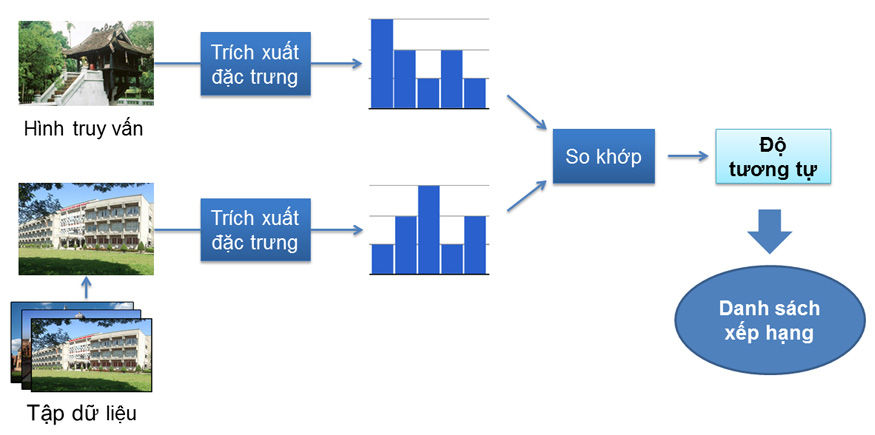
\includegraphics[scale=0.34]{overall}
    \else
      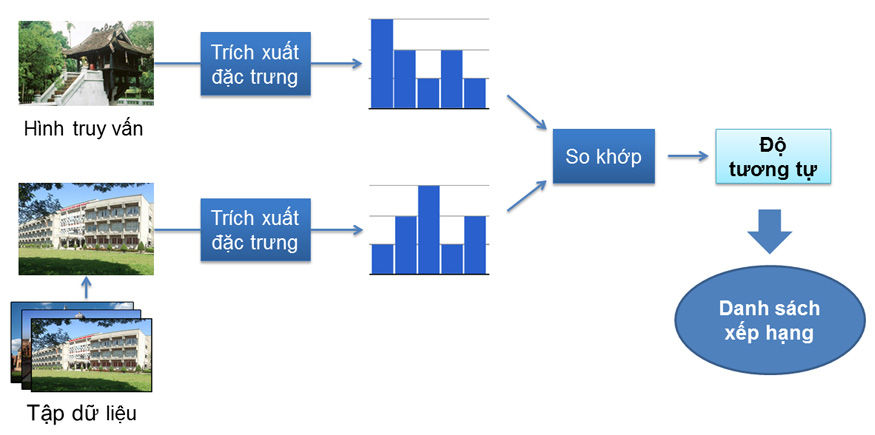
\includegraphics[scale=0.34]{overall}
    \fi
    \caption[Mô hình tổng quan của một hệ thống truy vấn ảnh]{Mô hình tổng quan của một hệ thống truy vấn ảnh.}
    \label{FigOverall}
  \end{center}
\end{figure}

\section{Rút trích đặc trưng hình ảnh}
\label{feature-extraction}
Trong lĩnh vực Thị giác Máy tính, một câu hỏi và cũng là một thách thức lớn đối với tất cả các nhà khoa học là làm sao biểu diễn được môt hình ảnh trên máy tính. Tùy theo từng mục đích cụ thể, người ta sẽ có các cách biểu diễn khác nhau. Trong truy vấn ảnh, một hình ảnh phải được biểu diễn dưới dạng sao cho bền vững trước những thay đổi như điều kiện chụp, tỉ lệ, góc chụp khác nhau hay thậm chí là những thay đổi lớn do đối tượng bị che khuất. Do sự tác động của các yếu tố này, cho dù hai hình ảnh chứa cùng một đối tượng thì vẫn có thể tồn tại một vùng hình ảnh lớn bên ngoài các đối tượng không đồng thời xuất hiện ở cả hai hình. Điều này gây khó khăn cho việc so khớp các hình ảnh.

Trong phần này, chúng tôi sẽ trình bày về hai hướng tiếp cận phổ biến được dùng để giải quyết vấn đề. Đó là hướng tiếp cận dựa trên đặc trưng toàn cục và đặc trưng cục bộ.

\subsection{Đặc trưng toàn cục}
Để nhận biết các vật thể quanh ta bằng thị giác, ta thường dựa trên các đặc trưng dễ nhận thay bằng mắt thường như màu sắc, hình dạng hay texture bề ngoài của vật. Đó chính là những đặc trưng toàn cục gần gũi nhất với thị giác của con người. Trong mục này, chúng tôi sẽ lần lượt trình bày các công trình nghiên cứu về những đặc trưng toàn cục cơ bản sử dụng trong truy vấn ảnh đó là: đặc trưng hình dạng, đặc trưng về texture và đặc trưng màu sắc.

\subsubsection{Đặc trưng hình dạng}
Hình dạng là một trong những đặc trưng quan trọng có thể nhìn thấy và cũng là một đặc trưng cơ bản để mô tả nội dung của hình ảnh. Tuy nhiên, biểu diễn và mô tả hình dạng của đối tượng trên ảnh là một việc vô cùng khó khăn bởi vì khi một đối tượng không gian ba chiều được được chiếu lên mặt phẳng không gian hai chiều sẽ làm mất đi một chiều thông tin của đối tượng. Do đó, hình dạng của đối tượng rút trích được từ hình ảnh thường chỉ thể hiện được một phần hình dạng của đối tượng. Ngoài ra, còn một vài khó khăn nữa phải đối mặt trong việc rút trích đặc trưng về hình dạng như về độ nhiễu, sự mất mát thông tin hình ảnh, sự che khuất hay méo mó, v.v...

Các kỹ thuật biểu diễn và mô tả hình dạng thường được chia làm hai dạng:\\
\textbf{Biểu diễn hình dạng dựa trên đường viền.} Kỹ thuật này chỉ tập trung khai thác thông tin về hình dạng đường biên của đối tượng trên ảnh. Nó được chia ra làm hai loại là tiếp cận liên tục và tiếp cận rời rạc. 

\begin{itemize}

\item Tiếp cận liên tục: là không chia hình dạng thành nhiều phần nhỏ, thông thường một vector sẽ được rút ra từ toàn bộ đường bao dùng để mô tả hình dạng. Và độ tương đồng giữa các hình dạng sẽ được đo bằng cách tính khoảng cách giữa các vector này.

Các bộ mô tả đơn giản phổ biến bao gồm \textit{diện tích}, \textit{độ tròn} ($C^2/S$, trong đó C là chu vi, S là diện tích), \textit{tính tâm sai} (chiều dài của trục lớn / chiều dài của trục nhỏ), \textit{hướng của trục chính}, \textit{lượng uốn cong} (bending energy)\cite{young1974analysis}. Những bộ mô tả đơn giản này thường chỉ có thể phân biệt hình dạng sai khác lớn, do đó chúng thường được dùng để lọc những trường hợp sai và kết hợp với những bộ mô tả hình dạng khác để phân biệt các hình dạng. Những bộ mô tả hình dạng đường viền khác được đề xuất bởi Peura and Iivarinen\cite{peura1997efficiency} bao gồm độ lồi, tỉ lệ của các trục cơ bản, phương sai đường tròn và phương sai elip.

Một phương pháp khác cũng được dùng phổ biến là phương pháp so khớp dựa trên sự tương xứng hình dạng. Phương pháp này ngược với kỹ thuật biểu diễn hình dạng dựa trên đặc trưng, tức là nó đo độ tương tự giữa các hình dạng sử dụng so khớp từng điểm. Nói cách khác, mọi điểm trên hình dạng được coi như các điểm đặc trưng. Việc so khớp được thực hiện trên không gian 2D. Một trong những phương pháp so khớp dựa trên sự tương xứng hình dạng cổ điển là phương pháp \textit{Hausdorff distance}\cite{chetverikov1999matching}. Nó thường dùng để xác định vị trí của đối tượng trên hình ảnh và đo độ tương đồng giữa các hình.

Ngoài những phương pháp trên, còn có các phương pháp khác như \textit{shape signature}\cite{davies2004machine, van1991contour, zhang2002comparative}, \textit{boundary moments}\cite{sonka2014image, gonzalez2002digital} , \textit{elastic matching}\cite{del1997visual}, \textit{scale space method}\cite{asada1986curvature},...

\item Tiếp cận rời rạc: là chia nhỏ hình dạng thành nhiều đoạn dựa trên một tiêu chuẩn đặc biệt, các đoạn được gọi là các hình cơ bản (primitives). Biểu diễn cuối cùng sẽ là một chuỗi ký tự, một biểu đồ (hoặc cây). Độ tương đồng giữa các hình dạng sẽ được đo bằng cách so khớp các chuỗi hoặc biểu đồ đó. Các phương pháp phổ biến dựa trên tiếp cận rời rạc phổ biến gồm \textit{polygonal approximation}, \textit{curvature decomposition} và \textit{curve fitting}\cite{pavlidis1982algorithms}.
\end{itemize}
\textbf{Biểu diễn hình dạng dựa trên vùng.} Trong kỹ thuật này, tất cả các pixel nằm trên vùng hình dạng của đối tượng được xử lý để thu được một dạng biểu diễn hình dạng thay vì chỉ dựa trên thông tin đường biên như các phương pháp dựa trên đường viền đã trình bày ở mục trước. Các phương pháp dựa trên vùng sử dụng các bộ mô tả mômen để mô tả hình dạng như \textit{geometric moment invariants}\cite{hu1962visual}, \textit{algebraic moment invariants}\cite{taubin1991recognition, taubin1991object}, \textit{orthogonal moments}\cite{teague1980image}. Ngoài ra còn một số phương pháp mô tả dựa trên vùng khác như grid method, shape matrix, convex hull và media axis. Tương tự như các phương pháp dựa trên đường viền, các hình dạng dựa trên vùng có thể được tạo thành theo thứ tự bất kỳ và bất biến trước các biến đổi afin. Tuy nhiên, trong công trình \cite{meier1998automatic}, tác giả Meier đã chỉ ra rằng những mômen đại số bất biến cho kết quả tất tốt hoặc rất xấu trên từng đối tượng truy vấn. Chúng cho kết quả tốt trên các đối tượng mà các pixel phân tán chứ không phải là viền của đối tượng.

\subsubsection{Đặc trưng texture}
Tương tự như hình dạng, texture là một trong những đặc trưng quan trọng để mô tả và nhận dạng hình ảnh. Điều này đã được chứng minh qua rất nhiều công trình nghiên cứu về phân tích texture của hình ảnh\cite{tuceryan1998texture, manjunath1996texture, montoya2009wavelet, xu2006evaluation}.

Texture có thể dễ dàng nhận biết trên hình ảnh. Ví dụ các texture thường thấy như cát, kim loại, gỗ, v.v... Tuy nhiên để một định nghĩa chuẩn cho nó thì không hề dễ dàng. Không giống như màu sắc, texture rất khó để phân tích nếu chỉ dựa trên giá trị của các pixel độc lập bởi  mà phải đặt trong mối quan hệ với các pixel xung quanh. Do đó ta có thể nêu ra được các thuộc tính của texture. Theo công trình \cite{tamura1978textural}, texture có các thuộc tính như độ thô ráp, độ tương phản, hướng, tính đều đặn, tính thô,...

Việc rút trích đặc trưng về texture có thể phân thành các hướng tiếp cận sau:\\
\textbf{Phương pháp thống kê.} Đây là một trong những cách truyền thống để phân tích được sự phân bố của độ xám trong không gian, chẳng hạn như tính toán xác suất xuất hiện của các giá trị độ xám ở các khoảng cách và hướng khác nhau. Việc thống kê có thể được thực hiện trên những giá trị của các pixel độc lập hoặc trên giá trị các cặp pixel\cite{tuceryan1998texture}. Các phương pháp biểu diễn texture bằng histogram cũng sử dụng những thông tin thống kê về texture. Một trong những phương pháp thống kê phổ biến nhất hiện nay là \textit{co-occurrence matrix}\cite{haralick1973textural}.\\
\textbf{Phương pháp hình học.} Phương pháp này phân tích texture bằng những thành phần gốc tạo nên texture. Sự phân tích đó dựa trên các thuộc tính hình học như kích cỡ, hình dáng, diện tích và độ dài. Sau khi xác định được những thành phần gốc đó trên hình ảnh, các quy luật sắp đặt sẽ được rút trích từ đó\cite{nevatia1982machine}. Tuy nhiên, các này không thể áp dụng cho những texture từ tự nhiên bởi vì những thành phần gốc và các luật sắp đặt có thể không phổ biến.\\
\textbf{Phương pháp dựa trên mô hình.} Phương pháp này ứng dụng kỹ thuật xây dựng mô hình cho hình ảnh để mô tả và tổng hợp texture. Các thông số của mô hình sẽ lưu lại các thành phần trực giác của texture\cite{tuceryan1998texture}. Ví dụ, các thành phần của texture có thể được mô hình như sau:các chấm đen và chấm sáng, sự dịch chuyển ngang hoặc dọc, các góc, các đường, v.v... Các bộ mô tả thuộc phương pháp này làm việc tốt với những texture phổ biến. Bộ mô tả \textit{local binary pattern} là một ví dụ cho bộ mô tả dựa trên mô hình.\\
\textbf{Phương pháp xử lý tín hiệu.} Các phương pháp xử lý tín hiệu mô tả texture bằng cách sử dụng các bộ lọc trên toàn hình ảnh. Cả bộ lọc theo không gian và tần suất cũng có thể được sử dụng. Các bộ mô tả dựa trên wavelet và Gabor đều thuộc phương pháp này. Ví dụ, \textit{homogeneous texture descriptor}\cite{wu2000texture, manjunath1996texture} là một bộ mô tả như vậy.

\subsubsection{Đặc trưng màu sắc}
Một trong những thuộc tính quan trọng nhất của đối tượng có thể nhìn thấy bằng mắt thường là màu sắc bởi vậy nó là một trong những thuộc tính quan trọng được sử dụng trong các hệ thống truy vấn dựa trên nội dung ảnh.

Các hướng tiếp cận về đặc trưng màu sắc có thể chia làm 3 dạng:\\
\textbf{Hướng tiếp cận tổng thể.} Hướng tiếp cận này xem xét các đặc trưng dưới góc độ tổng thể, do đó trong quá trình rút trích không hề có sự chia nhỏ hay tiền xử lý. Các bộ mô tả theo hướng này thường sử dụng những thuật toán đơn giản và nhanh gọn để rút trích các vector đặc trưng. Tuy nhiên, các thông tin về sự phân bố không gian của các màu sắc bị bỏ qua nên làm cho các bộ mô tả đó có ít giá trị trong việc phân tách hình ảnh. Có rất nhiều hướng tiếp cận tổng quan sinh ra các histogram hay các vector đặc trưng như \textit{global color histogram}\cite{swain1991color} và \textit{cumulative global color histogram}\cite{stricker1995similarity}.\\
\textbf{Hướng tiếp cận dựa trên các vùng có kích thước cố định.} Hướng tiếp cận này chia hình ảnh thành các ô với kích thước cố định và rút trích thông tin màu sắc từ mỗi ô một cách độc lập. Các bộ mô tả dựa trên phương pháp này càng mã hóa nhiều thông tin ảnh thì chi phí sẽ càng tăng. Một vài bộ mô tả dựa trên hướng tiếp cận này như: \textit{local color histogram}\cite{swain1991color} và \textit{cell/color histogram}\cite{stehling2003cell}.\\
\textbf{Hướng tiếp cận dựa trên sự phân đoạn.} Hướng tiếp cận này chia hình ảnh thành nhiều vùng, các vùng có thể có kích cỡ và số lượng khác nhau với các hình khác nhau. Quá trình phân chia này được thực hiện bởi một thuật toán chia đoạn hoặc gom cụm, điều này làm gia tăng chi phí tính toán cho quá trình rút trích đặc trưng. Một loại khác của sự phân đoạn là phân lớp các pixel trước khi rút trích đặc trưng. Các bộ mô tả dựa trên hướng tiếp cận này thường cho kết quả tốt hơn mặc dù chi phí tính toán cao hơn. Một số ví dụ về các bộ descriptor dựa trên phương pháp chia đoạn như \textit{color-based clustering}\cite{stehling2003cell} và \textit{dominant-color}\cite{deng2001efficient, manjunath2001color}.

Mặc dù các đặc trưng toàn cục kể trên đều là những đặc trưng quan trọng nhất để nhận diện hình ảnh nhưng các hướng tiếp cận dựa trên các đặc trưng toàn cục vẫn chưa đạt được kết quả cao trong phân lớp và truy vấn ảnh. Một trong những hướng tiếp cận thu hút được nhiều sự chú ý và đạt được nhiều kết quả triển vọng trong những năm gần đây đó là tiếp cận dựa trên đặc trưng cục bộ. Chúng tôi sẽ trình bày chi tiết về hướng tiếp cận này ở phần kế tiếp.


\subsection{Đặc trưng cục bộ}
\label{local-features}

Trong những năm gần đây, rất nhiều công trình nghiên cứu đã khai thác các đặc trưng cục bộ để biểu diễn hình ảnh phục vụ cho các bài toán về truy vấn và phân lớp ảnh và đã đạt được những thành quả đáng khích lệ.

Bản chất của hướng tiếp cận này là rút trích những "chi tiết" cục bộ (local patches) trên tấm hình để biểu diễn cho hình ảnh đó. Hướng tiếp cận này được đưa ra dựa trên nhận định rằng hai hình ảnh tương tự nhau sẽ có rất nhiều những chi tiết cục bộ giống nhau và những chi tiết cục bộ này có thể được dùng để so khớp các hình ảnh với nhau. Các chi tiết này thường được rút trích bằng một trong hai phương pháp, đó là: (i) sử dụng một lưới dày đặc với nhiều mức tỉ lệ kích cỡ khác nhau (để đảm bảo bất biến về tỉ lệ) để chia hình ảnh thành nhiều chi tiết nhỏ, hoặc (ii) dùng các phương pháp dò tìm (detector) hay một kỹ thuật nào đó để lấy được các chi tiết đặc biệt (đặc trưng) trên vùng hình ảnh quan tâm và đồng thời loại bỏ những chi tiết không đảm bảo sự bất biến tỉ lệ ngay ở bước này. Có thể thấy rằng phương pháp dùng lưới để chia hình ảnh thành nhiều phần không thể áp dụng cho bài toán truy vấn ảnh với tập dữ liệu lớn vì ta cần rất nhiều không gian để lưu trữ một lượng lớn các chi tiết dày đặc với nhiều mức tỉ lệ kích cỡ khác nhau. Do vậy phương pháp biểu diễn hình ảnh bằng các đặc trưng được áp dụng cho bài toán này.

Có rất nhiều phương pháp dò tìm các điểm đặc trưng (feature detector) được đưa ra, trong đó phải kể tới các phương pháp được dùng phổ biến như Difference of Gaussians, DoG \cite{lowe2004distinctive}, Maximally Stable Extremal Regions, MSER \cite{matas2004robust} và affine invariant detector \cite{mikolajczyk2004scale}. Ngoài ra còn có các phương pháp dò tìm được xây dựng để tìm kiếm trong thời gian thực như SURF \cite{bay2006surf}, FAST \cite{rosten2010faster} và BRISK \cite{leutenegger2011brisk}.

Sau khi rút trích được các điểm đặc trưng cục bộ cho mỗi hình, dựa trên các đặc trưng đó ta sẽ quyết định xem liệu hai tấm hình bất kỳ có chứa cùng một đối tượng hay không. Để so sánh độ tương đồng của hai đặc trưng cục bộ, ta không thể dựa trên màu sắc và cường độ của chúng vì những yếu tố này không bền vững trước những thay đổi của hình ảnh. Do đó ta cần phải tìm cách lượng tử hóa độ tương đồng giữa cách đặc trưng để có thể đo được bằng các tính toán cụ thể. Trong công trình nghiên cứu nổi tiếng của Lowe \cite{lowe2004distinctive}, tác giả đã đề xuất một phương pháp để có thể tính toán được một bộ mô tả (descriptor) có tính phân loại cao và đảm bảo sự bất biến trước những thay đổi của hình ảnh, đó là SIFT descriptor. Theo sau công trình nghiên cứu này, nhiều công trình có hướng tiếp cận tương tự được đưa ra, trong đó bao gồm GLOH \cite{mikolajczyk2005performance}, SURF \cite{bay2006surf}, DAISY \cite{tola2008fast}, CONGAS \cite{zheng2009tour}, BRIEF \cite{calonder2010brief}. Đặc biệt, bằng việc đề xuất thuật toán RootSIFT được cải tiến từ SIFT, Arandjelovic và Zisserman \cite{arandjelovic2012three} đã nâng hiệu suất của phương pháp SIFT lên đáng kể. Đây cũng là phương pháp được chúng tôi chọn dùng trong hệ thống của mình.

Tóm lại, từ những bộ mô tả (descriptor) được rút trích từ tất cả các hình trong cơ sở dữ liệu và từ hình ảnh truy vấn, ta có thể tính toán được độ tương đồng giữa các hình ảnh. Tuy nhiên, hiệu suất của quá trình tính toán độ tương đồng bị giảm đi đáng kể khi thực hiện trên tập dữ liệu lớn. Trong phần tiếp theo, chúng tôi sẽ giới thiệu sơ lược về một mô hình giúp giải quyết được vấn đề này.

\section{Biểu diễn hình ảnh bằng mô hình Bag-of-words}
\label{bag-of-words}
Trong truy vấn hình ảnh, Bag-of-words (BoW) là mô hình biểu diễn hình ảnh được sử dụng phổ biến nhất hiện nay và đạt được những kết quả rất tốt, chẳng hạn như công trình cho kết quả tốt nhất hiện nay của Arandjelovic và Zisserman\cite{arandjelovic2012three} cũng sử dụng mô hình này. Hình \ref{FigBoWPreview} minh họa ý tưởng biểu diễn hình ảnh với mô hình BoW.

\begin{figure}[!htbp]
  \begin{center}
    \leavevmode
    \ifpdf
      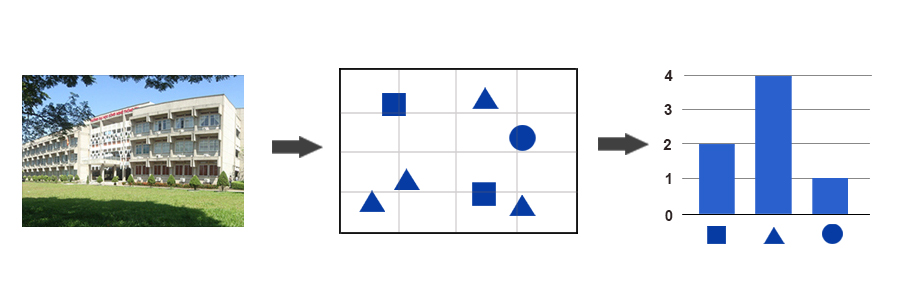
\includegraphics[scale=0.45]{bow-preview}
    \else
      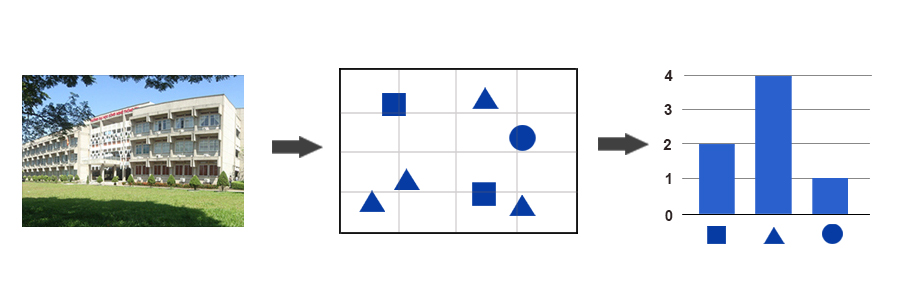
\includegraphics[scale=0.45]{bow-preview}
    \fi
    \caption[Biểu diễn hình ảnh bằng mô hình Bag-of-words]{Biểu diễn hình ảnh bằng mô hình Bag-of-words.}
    \label{FigBoWPreview}
  \end{center}
\end{figure}

Mô hình BoW được ứng dụng từ lĩnh vực xử lý văn bản, với ý tưởng biểu diễn một hình ảnh như một văn bản. Cụ thể hơn, BoW biểu diễn các đặc trưng cục bộ bằng các visual word, và từ những visual word sẽ xây dựng được một histogram biểu diễn hình ảnh đó. Như đã giới thiệu trong Mục \ref{local-features}, một hình ảnh có thể rút trích được các đặc trưng cục bộ, tuy nhiên các đặc trưng này lại hoàn toàn phân biệt với nhau, vậy làm thế nào để xây dựng được các visual word từ các đặc trưng này? Hình \ref{FigBoW} cho thấy các bước xử lý trong mô hình BoW.

\begin{figure}[!htbp]
  \begin{center}
    \leavevmode
    \ifpdf
      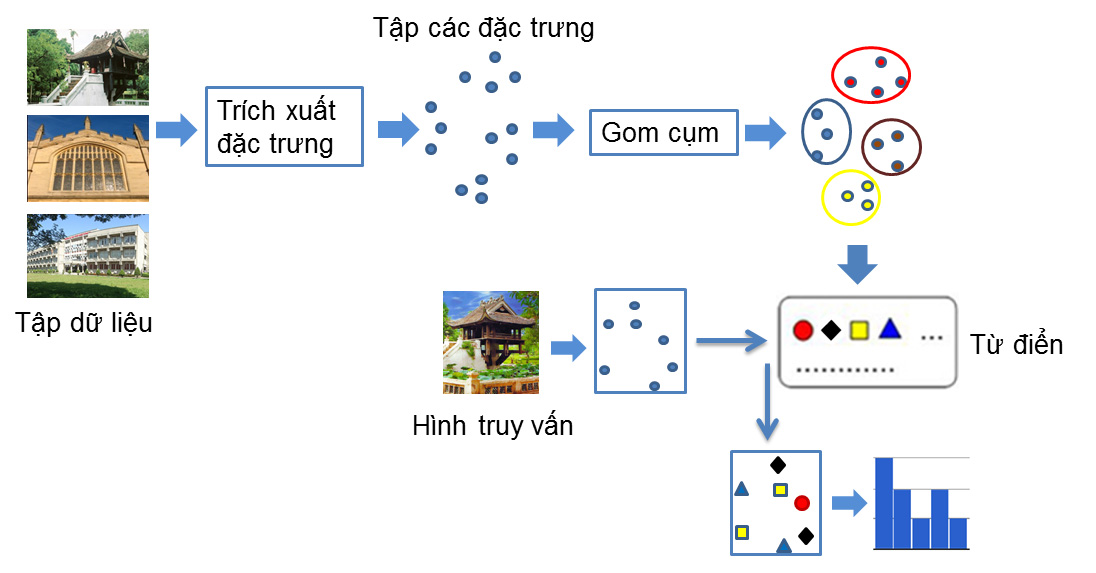
\includegraphics[scale=0.38]{bow}
    \else
      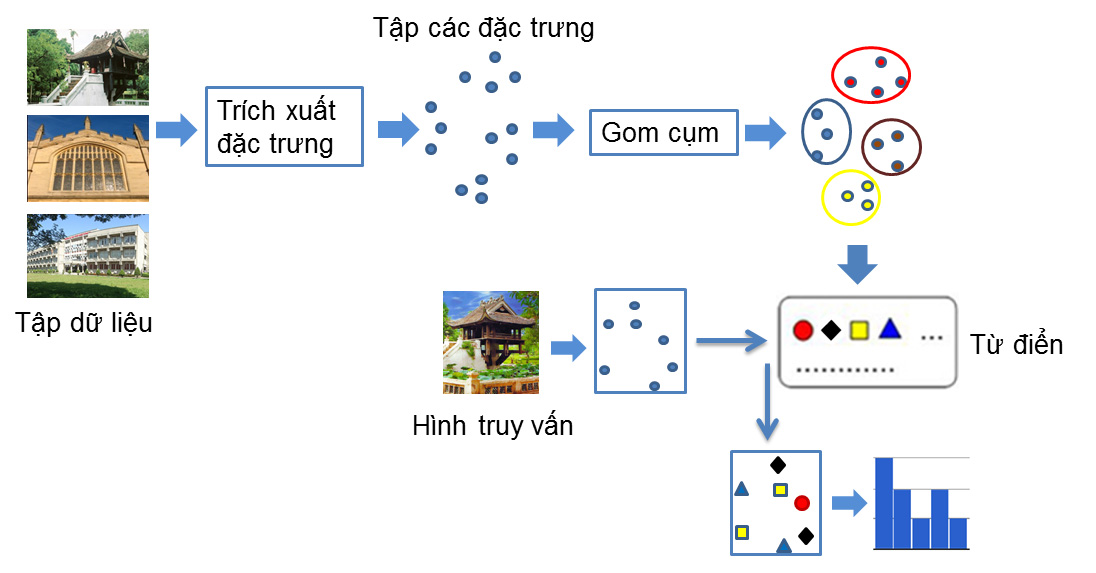
\includegraphics[scale=0.38]{bow}
    \fi
    \caption[Mô hình Bag-of-words]{Mô hình Bag-of-words.}
    \label{FigBoW}
  \end{center}
\end{figure}

Nghiên cứu của Sivic và Zisserman \cite{sivic2003video} là công trình đầu tiên ứng dụng hướng tiếp cận trong xử lý văn bản vào truy vấn ảnh\footnote{Mục đích của tác giả trong nghiên cứu này là truy vấn trên video nhưng ta hoàn toàn có thể chuyển sang bài toán truy vấn ảnh bằng cách rút trích các frame trong video theo từng giây}. Trong công trình này tác giả đã giới thiệu khái niệm visual word, được tạo ra bằng cách sử dụng thuật toán gom cụm K-Means để gom cụm các đặc trưng cục bộ. Hình \ref{FigVisualWords} cho thấy một vài ví dụ về các visual word. Tương tự như trong truy vấn văn bản, hình ảnh sẽ được rút trích các đặc trưng cục bộ rồi tiếm hành gom cụm các đặc trưng này sẽ thu được các visual word. Tập các visual word này được gọi là một bộ từ điển. Khi một hình ảnh được đưa vào từ điển, mỗi đặc trưng của nó sẽ được đánh chỉ số theo visual word có khoảng cách gần nhất với đặc trưng đó.

\begin{figure}[!htbp]
  \begin{center}
    \leavevmode
    \ifpdf
      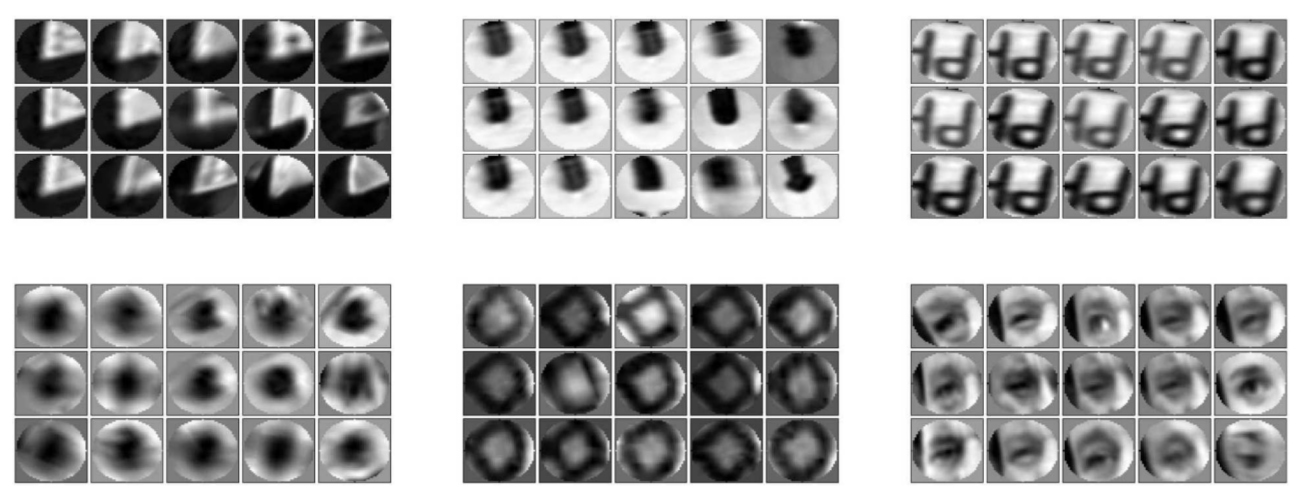
\includegraphics[scale=0.32]{visualWords}
    \else
      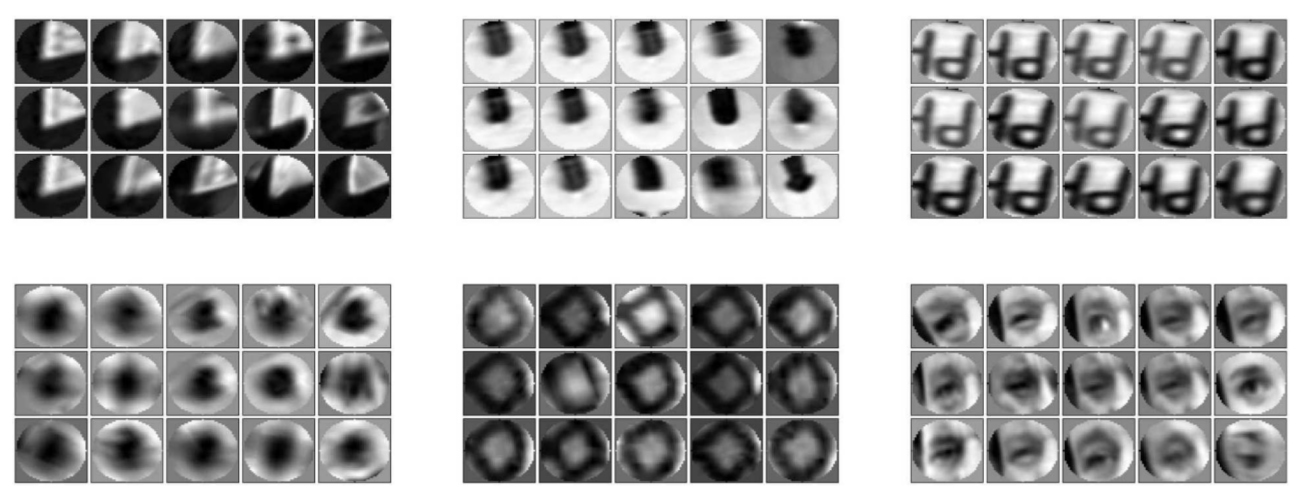
\includegraphics[scale=0.32]{visualWords}
    \fi
    \caption[Các từ visual word]{\textbf{Các visual word.} Mỗi nhóm là một nhóm các đặc trưng cục bộ được rút trích từ hình ảnh, gom vào cùng một cụm và cùng được biểu diễn bằng một visual word. Hình ảnh được lấy từ bài báo \cite{sivic2009efficient}.}
    \label{FigVisualWords}
  \end{center}
\end{figure}

Thí nghiệm trong công trình của của Sivic và Zisserman \cite{sivic2003video} được tiến hành trên 4000 ảnh (frame) được lấy từ video, sử dụng 10,000 visual word được gom cụm từ các đặc trưng cục bộ của các hình ảnh đó.Trong thực tế, để truy vấn ảnh trên những tập dữ liệu lớn, để cho kết quả tốt thì số lượng visual word không thể vào khoảng 10,000 từ mà phải lên tới hàng triệu từ\cite{philbin2007object}. Trong khi đó, độ phức tạp của thuật toán K-Means là \textit{O(N\textsubscript{w}N\textsubscript{d})} với N\textsubscript{w}, N\textsubscript{d} lần lượt là kích cỡ của visual word và số tập của bộ mô tả huấn luyện (training descriptor set). Trên những tập dữ liệu lớn thì N\textsubscript{d} $\geq$ N\textsubscript{w} nên độ phức tạp luôn lớn hơn $O(N^2_w)$. Do đó nếu dùng K-Means cho bài toán này chi phí tính tính toán sẽ vô cùng lớn. Nister và Stewenius \cite{nister2006scalable} đã đề xuất phương pháp giải quyết cho bài toán này bằng cách xây dựng một cây từ vựng mà về bản chất thì nó chính là thuật toán Hierarchical K-Means (HKM). Để minh họa cho thuật toán này, tác giả đã cho thử nghiệm trên bộ ảnh gồm 1 triệu hình ảnh. Không lâu sau đó, Philbin và các đồng nghiệp \cite{philbin2007object} đã đề xuất một hướng tiếp cận khác dựa trên thuật toán \textit{xấp xỉ K-Means}, Approximate K-Means (AKM). Tác giả cũng cho chạy thử nghiệm AKM trên 16.7 triệu đặc trưng để gom cụm thành 1 triệu từ. Các thí nghiệm cho thấy rằng, khi so sánh AKM với K-Means thì về độ chính xác thì AKM xấp xỉ K-Means tuy nhiên chi phí tính toán chỉ bằng một phần nhỏ của K-Means. Còn khi so sánh AKM với HKM thì AKM không những vượt xa về độ chính xác mà còn có thể áp dụng cho những tập dữ liệu lớn. Chi phí tính toán của cả HKM và AKM đều là $O(N_d log(N_w))$.

\section{So khớp hình ảnh}
\label{matching}
Quá trình so khớp hình ảnh phụ thuộc phần lớn vào việc hình ảnh đã được biểu diễn như thế nào. Với mô mình BoW như đã trình bày tại Mục \ref{bag-of-words}, mỗi hình ảnh sẽ trở thành một histogram, khoảng cách giữa các histogram này thể hiện độ tương tự giữa các hình ảnh. Thêm vào đó, các histogram này cần được đánh trọng số thích hợp để tăng độ chính xác truy vân. Cũng giống như mô hình BoW trong xử lý văn bản, \textit{tf-idf}\cite{manning2008introduction} là phương pháp tiêu chuẩn để đánh trọng số. \textit{Tf-idf} trong xử lý văn bản được định nghĩa như sau:

Giả sử với bộ từ điển gồm \textit{k} từ, mỗi từ sẽ được biểu diễn bằng một vector k chiều $V_i = (t_1, t_2, ..., t_i, ..., t_k)^T$, với:

\begin{eqnarray}
t_i = \frac{n_{id}}{n_d}log\frac{N}{n_i}
\end{eqnarray}
trong đó, $n_{id}$ là số lần xuất hiện của từ $i$ trong văn bản $d$, $n_d$ là tổng số từ trong văn bản $d$, $n_i$ là số lần xuất hiện của từ $i$ trong toàn bộ từ điển và $N$ là tổng số văn bản trong từ điển. Phương pháp đánh trọng số này gồm hai thành phần chính là \textit{tf} (\textit{term frequency}) là tần số xuất hiện của từ trong văn bản ($\frac{n_{id}}{n_d}$) thể hiện mức độ quan trọng của từ đó trong văn bản và \textit{idf} (\textit{inverse document frequency}) thể hiện mức độ ảnh hưởng của từ đó tới toàn bộ dữ liệu. Một từ có thể có mức độ quan trọng cao nếu nó xuất hiện nhiều lần trong một văn bản, nhưng nếu nó xuất hiện trong hầu hết các văn bản thì nó lại không có ý nghĩa nhiều để phân loại hoặc so sánh các văn bản với nhau.

Trong truy vấn và phân loại hình ảnh sử dụng mô hình BoW, tf-idf được sử dụng tương tự như trên để đánh trọng số cho các histogram biểu diễn hình ảnh, với các từ là các visual word và các văn bản là các hình ảnh. Sau đó, khoảng cách giữa các histogram được tính bằng một trong các độ đo phổ biến: $L_1$ distance\cite{krauss1987taxicab}, Euclidean distance ($L_2$)\cite{deza2009encyclopedia} và histogram intersection (HI)\cite{cheng2010mammographic}.
\\
\\
\textbf{L1 distance}

L1 distance là độ đo khoảng cách cơ bản giữa hai vector. Khoảng cách $d$ giữa hai vector $p$, $q$ được tính như sau:

\begin{eqnarray}
d(p,q) = d(q,p) = ||p-q|| = \sum\limits_{i=1}^n |p_i - q_i|
\end{eqnarray}

Trong đó $p = (p_1, p_2, p_3, ..., p_n)$ và $q = (q_1, q_2, q_3, ..., q_n)$
\\
\\
\textbf{L2 distance}

L2 distance là độ đo khoảng cách được sử dụng khá phổ biến và cho kết quả tốt trong nhiều trường hợp, được tính như sau:

\begin{eqnarray}
d(p,q) = d(q,p) = \sqrt{(q_1-p_1)^2 + ... + (q_n-p_n)^2} = \sqrt{\sum\limits_{i=1}^n (q_i - p_i)^2}
\end{eqnarray}
trong đó $p$, $q$ là các véc $n$ chiều, $p = (p_1, p_2, ..., p_n)$ và $q = (q_1, q_2, ..., q_n)$, $d(p,q)$ là khoảng cách giữa $p$ và $q$.
\\
\\
\textbf{Histogram Intersection}

Được đưa ra năm 2010 bởi Erkang Cheng và các đồng nghiệp\cite{cheng2010mammographic}, histogram intersection (HI) cũng thể hiện được hiệu quả của nó trong những trường hợp nhất định. Giá trị $S_{HI}$ thể hiện mức độ tương đồng giữa hai histogram $h_1$ và $h_2$ được định nghĩa như sau:

\begin{eqnarray}
S_{HI}(h_1, h_2) = \sum\limits_{i = 1}^n min(h_1(i), h_2(i))
\end{eqnarray}
Tác giả cũng đưa ra phương pháp Normalized HI (NHI):

\begin{eqnarray}
S_{NHI}(h_1, h_2) = \sum\limits_{i = 1}^n \frac{min(h_1(i), h_2(i))}{h_1(i) + h_2(i)}
\end{eqnarray}
cũng cho kết quả khả quan trong một số trường hợp khác.

Với ba độ đo trên ta có thể thấy, $L1$ và $L2$ thể hiện cả mức độ giống nhau và khác nhau giữa hai histogram, trong khi đó histogram intersection quan tâm chủ yếu tới mức độ giống nhau giữa hai histogram.
Việc sử dụng độ đo nào cho thích hợp tùy thuộc vào các trường hợp cụ thể, và nó còn liên quan tới nhiều vấn đề khác như kích thước từ điển ảnh hưởng tới kích thước mỗi histogram, mức độ thưa hay nhiễu của các histogram...

Trong truy vấn hình ảnh, quá trình so khớp được sử dụng khi có một hình truy vấn được đưa vào, nó sẽ được so khớp với các hình trong bộ dữ liệu. Để tăng tốc quá trình truy vấn, phương pháp chỉ mục ngược (inverted index) được sử dụng phổ biến và cho thấy hiệu quả cao giúp cải thiện hiệu suất truy vấn.

\section{Sử dụng thông tin về sự phân bố trong không gian ảnh của các đặc trưng}
\label{spatial}

Mặc dù đạt được những kết quả rất đáng chú ý nhưng mô hình BoW cơ bản vẫn bị giới hạn về độ chính xác do bỏ qua một thông tin quan trọng, đó là sự phân bố về không gian của các visual word. Do đó các đặc trưng cục bộ được xử lý một cách rời rạc, không liên quan tới nhau. Hình \ref{FigLimited} minh họa cho trường hợp các ảnh khác nhau được biểu diễn như nhau nếu không xem xét sự phân bố về không gian của các visual word.
\begin{figure}[!htbp]
  \begin{center}
    \leavevmode
    \ifpdf
      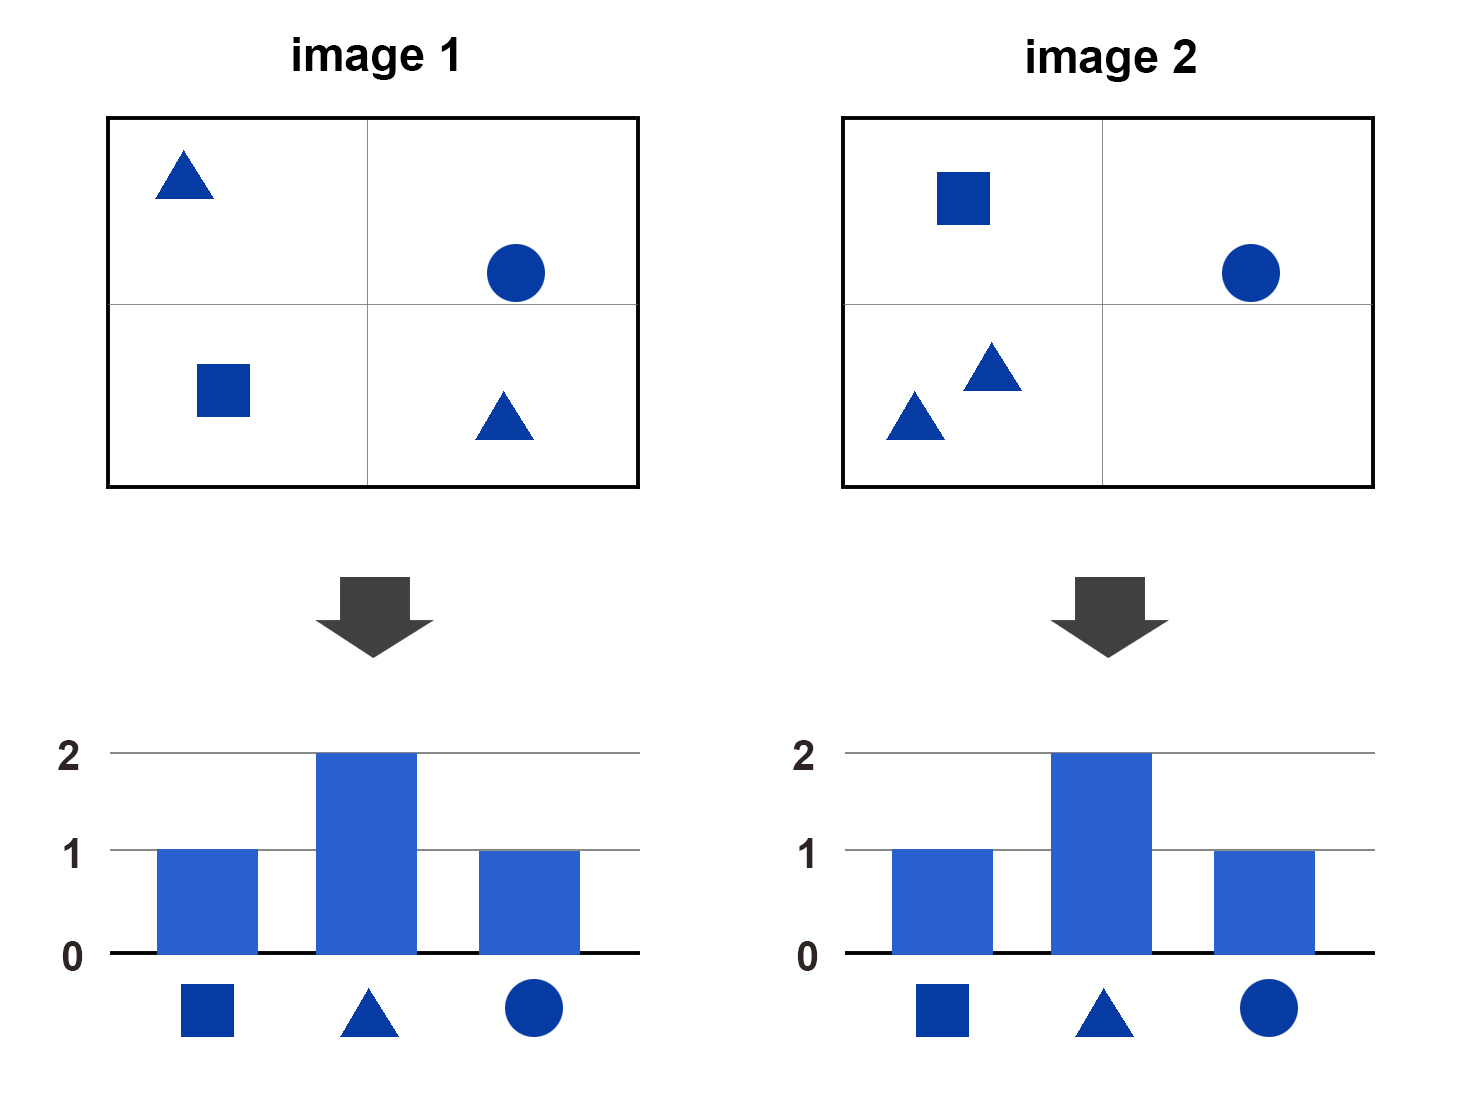
\includegraphics[scale=0.2]{limited}
    \else
      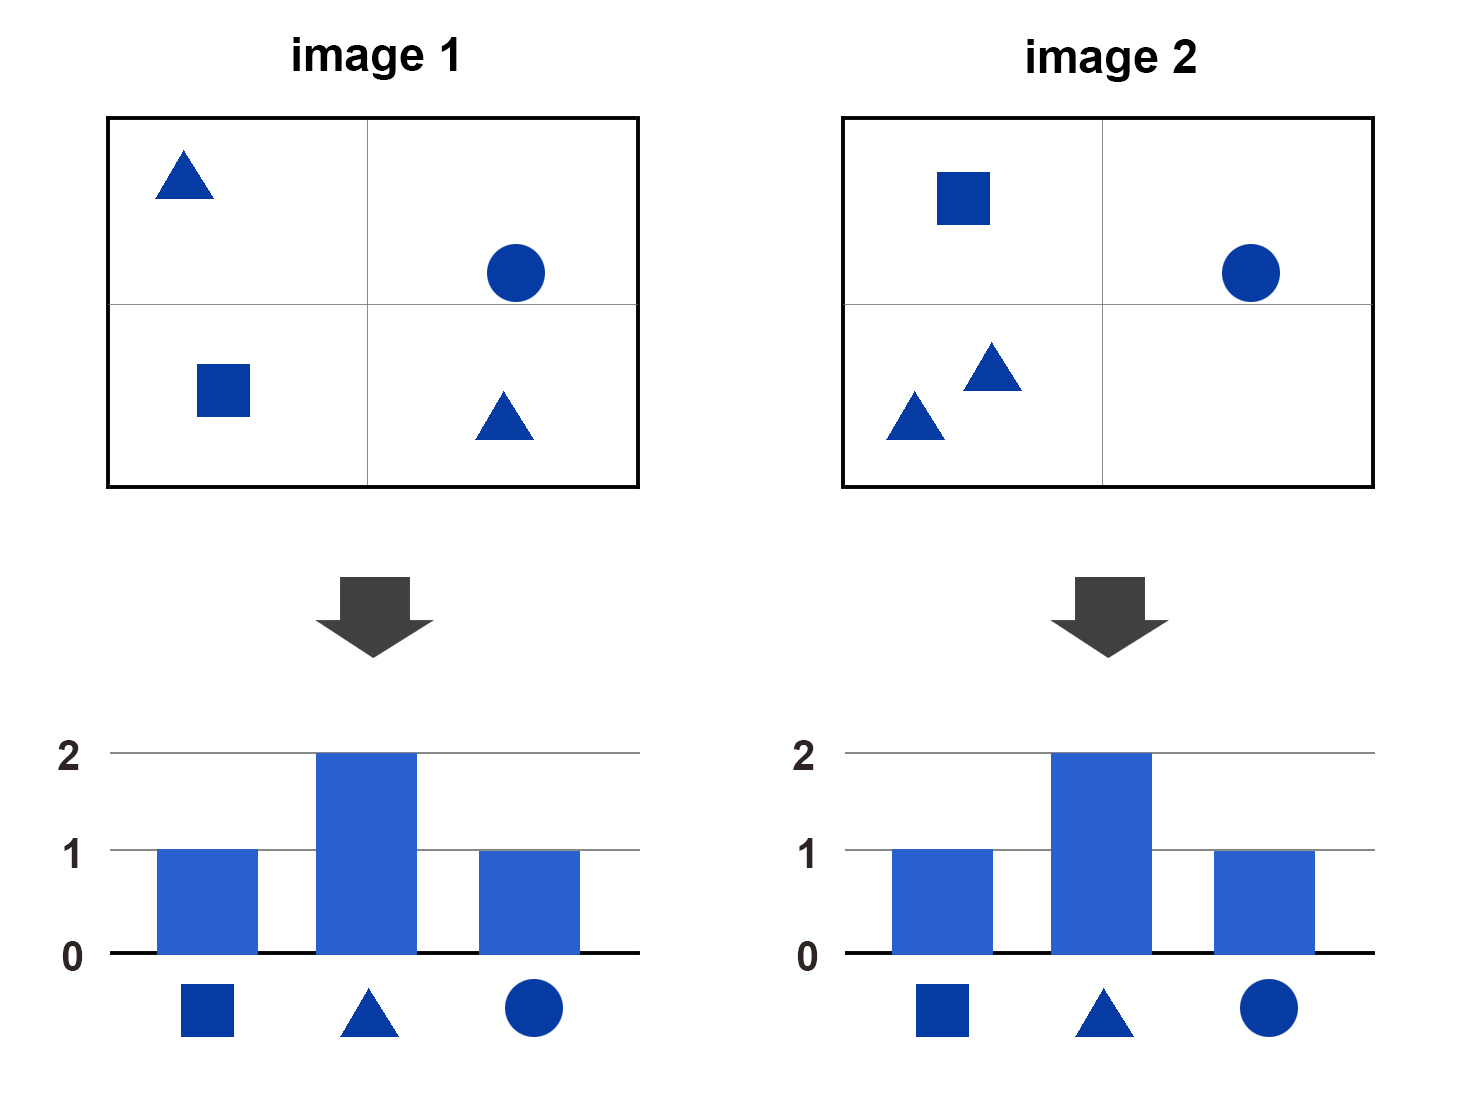
\includegraphics[scale=0.2]{limited}
    \fi
    \caption[Bỏ qua thông tin về sự phân bố trong không gian của các visual word trong mô hình BoW]{\textbf{Bỏ qua thông tin về sự phân bố trong không gian của các visual word trong mô hình BoW.} Sau khi được biểu diễn bằng mô hình BoW, hai hình ảnh trên được coi như giống nhau hoàn toàn trong khi chúng khác nhau do các visual word nằm ở các vị trí khác nhau.}
    \label{FigLimited}
  \end{center}
\end{figure}

Để giải quyết vấn đề trên, rất nhiều công trình nghiên cứu đã được đưa ra. Phần lớn các hướng tiếp cận được chia ra làm hai dạng là tiếp cận dựa trên đặc trưng hình học và tiếp cận dựa trên thông tin không gian của các điểm đặc trưng cục bộ. Trong mục \ref{geometry} chúng tôi sẽ trình bày về các phương pháp dựa trên đặc trưng hình học. Hướng tiếp cận còn lại sẽ được trình bày chi tiết trong mục \ref{spm}.

\subsection{Các hướng tiếp cận dựa trên đặc trưng hình học}
\label{geometry}
Các phương pháp sử dụng đặc trưng hình học để so khớp thường được dùng ở bước hậu xử lý để nhận dạng hình học. Dưới đây là một vài công trình tiêu biểu sử dụng hướng tiếp cận này.

Sivic và Zisserman \cite{sivic2003video} đã đo đạc sự nhất quán không gian cục bộ (local spatial consistency) trong các so khớp giữa hình ảnh truy vấn và từng hình ảnh trong cơ sở dữ liệu từ đó tái xếp hạng lại danh sách kết quả trả về. Việc đo đạc sự nhất quán không gian cục bộ trong so khớp hình ảnh cũng được đề cập tới trước đó trong các công trình như \cite{zhang1995robust} và \cite{schmid1997local}.

Trong một công trình nghiên cứu \cite{philbin2007object}, tác giả sử dụng thuật toán RANSAC \cite{fischler1981random} để kiểm tra sự nhất quán hình học giữa các đặc trưng cục bộ trùng khớp. RANSAC là một trong những phương pháp phổ biến nhất cho hậu xử lý toàn cục trên hình ảnh. Đặc biệt, trong một công trình khác, Zhang và các đồng nghiệp \cite{zhang2011image} đề xuất mã hóa thông tin không gian ảnh qua các mệnh đề trực quan hình học (GVP) kết hợp với RANSAC đã cho kết quả rất đáng chú ý với bộ dữ liệu lên tới hàng triệu ảnh.

Trong khi đó, công trình \cite{lin2010local} và \cite{lampert2009detecting} lại xếp hạng các hình ảnh dựa trên điểm số so khớp của hình ảnh truy vấn với những cửa sổ con được định vị trên hình. Phương pháp này mã hóa được nhiều thông tin không gian ảnh hơn so với mô hình BoW trên toàn bộ tấm hình và giúp định vị hình ảnh truy vấn.

Nhìn chung, những phương pháp sử dụng hướng tiếp cận hình học đều cho kết quả tốt. Tuy nhiên, khi vùng truy vấn lớn hơn thì chúng chỉ được dùng để tái xếp hạng một số lượng giới hạn ở các hình ảnh ở top đầu của kết quả trả về vì vấn đề về chi phí cho bộ nhớ và tốc độ thực hiện.

\subsection{Các hướng tiếp cận dựa trên thông tin không gian của các điểm đặc trưng cục bộ}
\label{spm}

Hướng tiếp cận dựa trên đặc trưng hình học là hướng tiếp cận mang tính toàn cục, tức là xem xét đối tượng dưới một cái nhìn tổng quan, toàn thể chứ không xem xét chi tiết những thành phần cấu thành nó. Hướng tiếp cận dựa trên các đặc trưng cục bộ lại ngược lại, xem đối tượng là một tập hợp của nhiều thành phần và dựa trên những thành phần đó để xác định đối tượng. Lazebnik \cite{lazebnik2006beyond} đã giới thiệu một phương pháp nền tảng, được bắt nguồn từ ý tưởng \textit{so khớp phân cấp} (pyramid matching) của Grauman và Darrell \cite{grauman2005pyramid}, đó là phương pháp \textit{so khớp không gian phân cấp} (Spatial Pyramid Matching - SPM). Ý tưởng của phương pháp này là lặp đi lặp lại việc chia nhỏ hình ảnh và tính toán biểu đồ của các đặc trưng cục bộ với mức độ chi tiết tăng dần. SPM đã giúp nâng cao một cách đáng kể độ chính xác cho mô hình BoW và tỏ ra là một phương pháp đơn giản nhưng hiệu quả. Mặc dù vậy, SPM cũng làm tăng thời gian thực hiện truy vấn bởi khi mức độ chi tiết càng cao thì kích cỡ biểu đồ của các đặc trưng cục bộ cũng tăng theo làm tăng chi phí tính toán trong quá trình so khớp, vì vậy SPM vẫn chưa thích hợp cho các bài toán yêu cầu thời gian thực.

\begin{figure}[!htbp]
  \begin{center}
    \leavevmode
    \ifpdf
      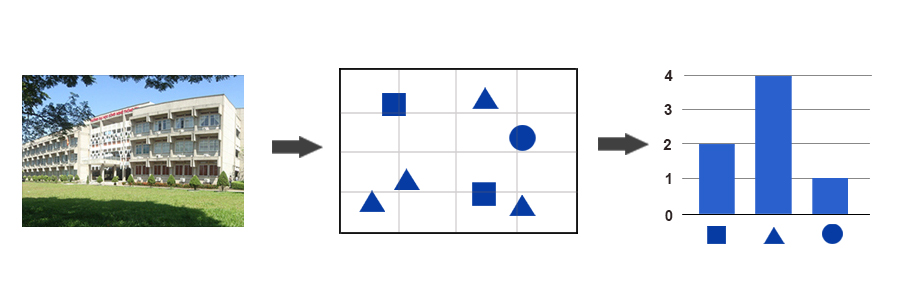
\includegraphics[scale=0.45]{bow-preview}
    \else
      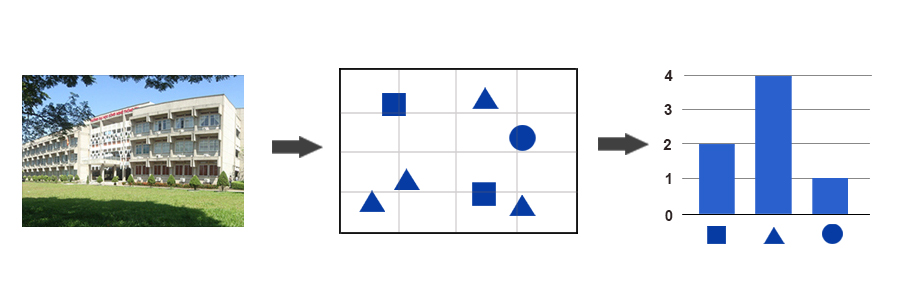
\includegraphics[scale=0.45]{bow-preview}
    \fi
    \caption[Phương pháp Spatial Pyramid Matching]{Phương pháp Spatial Pyramid Matching.}
    \label{FigSPM}
  \end{center}
\end{figure}

\section{Kết chương}

Việc biểu diễn hình ảnh bằng các đặc trưng cục bộ đã đặt nền tảng cho việc đưa ra các phương pháp để truy vấn đối tượng trên ảnh. Mô hình BoW đã chứng minh tính hiệu quả của mình trong truy vấn ảnh và việc kết hợp phương pháp chỉ mục ngược (inverted index) giúp giảm đáng kể thời gian thực hiện truy vấn. Tuy nhiên, mô hình BoW vẫn bị giới hạn về độ chính xác do bỏ qua thông tin không gian ảnh. Trong khi đó, rất nhiều hướng tiếp cận khác tận dụng được thông tin này đã nâng độ chính xác truy vấn nhưng lại cần chi phí tính toán cao, tốc độ phản hồi chậm.

Vì vậy, với những hạn chế trên, chúng tôi đề xuất một phương pháp tập trung vào việc cân bằng độ chính xác truy vấn và tốc độ phản hồi. 